%%%%%%%%%%%%%%%%%%%%%%%%%%% asme2ej.tex %%%%%%%%%%%%%%%%%%%%%%%%%%%%%%%
% Template for producing ASME-format journal articles using LaTeX    %
% Written by   Harry H. Cheng, Professor and Director                %
%              Integration Engineering Laboratory                    %
%              Department of Mechanical and Aeronautical Engineering %
%              University of California                              %
%              Davis, CA 95616                                       %
%              Tel: (530) 752-5020 (office)                          %
%                   (530) 752-1028 (lab)                             %
%              Fax: (530) 752-4158                                   %
%              Email: hhcheng@ucdavis.edu                            %
%              WWW:   http://iel.ucdavis.edu/people/cheng.html       %
%              May 7, 1994                                           %
% Modified: February 16, 2001 by Harry H. Cheng                      %
% Modified: January  01, 2003 by Geoffrey R. Shiflett                %
% Use at your own risk, send complaints to /dev/null                 %
%%%%%%%%%%%%%%%%%%%%%%%%%%%%%%%%%%%%%%%%%%%%%%%%%%%%%%%%%%%%%%%%%%%%%%

%%% use twocolumn and 10pt options with the asme2ej format
\documentclass[twocolumn,10pt]{asme2ej}

\usepackage{epsfig} %% for loading postscript figures
\usepackage{fixltx2e}
\usepackage{amsmath}
\usepackage{amsfonts}
\usepackage{cite}
\usepackage{array}
\usepackage{booktabs}
\usepackage{mathtools}
\usepackage{tabularx}
\usepackage{graphicx}
\usepackage{subfig}
\graphicspath{ {./images/} }
\pagenumbering{arabic}
\newcommand{\hquad}{\hspace{0.5em}}
%% The class has several options
%  onecolumn/twocolumn - format for one or two columns per page
%  10pt/11pt/12pt - use 10, 11, or 12 point font
%  oneside/twoside - format for oneside/twosided printing
%  final/draft - format for final/draft copy
%  cleanfoot - take out copyright info in footer leave page number
%  cleanhead - take out the conference banner on the title page
%  titlepage/notitlepage - put in titlepage or leave out titlepage
%  
%% The default is oneside, onecolumn, 10pt, final


\title{On the synthesis and design of a novel backdrivable high-stiffness capstan drive}

%%% first author
\author{Jordan M. Longval and Clément Gosselin
    \affiliation{
    Département de génie mécanique\\
	Université Laval\\
	1065 Avenue de la Médecine\\
	Québec, Qc G1V0A6\\
	Canada\\
	Jordan.Longval.1@ulaval.ca, Clement.Gosselin@gmc.ulaval.ca
    }	
}
   

\begin{document}

\maketitle    

%%%%%%%%%%%%%%%%%%%%%%%%%%%%%%%%%%%%%%%%%%%%%%%%%%%%%%%%%%%%%%%%%%%%%%
\begin{abstract}
{\it This article introduces a novel backdrivable high-stiffness cable capstan drive architecture for robotics applications. The drive has a low transmission ratio and a higher stiffness than typical capstan drives. The higher transmission stiffness is obtained by the use of grooves on both the input and the output pulleys of the drive which increases the effective coefficient of friction between the pulleys and the cable. The groove on the input pulley forms a single helix while the grooves on the output pulley form a $R$-helix, where $R$ is equal to the transmission ratio of the drive. This property enables several different multi-cable arrangements for the drive, which further increases the transmission stiffness. A kinematic model of the capstan drive is established and used to ensure the proper alignment of the input pulley groove and output pulley grooves as a function of the distance between the pulleys. A 3D printed prototype of the transmission is presented.
}
\end{abstract}

%%%%%%%%%%%%%%%%%%%%%%%%%%%%%%%%%%%%%%%%%%%%%%%%%%%%%%%%%%%%%%%%%%%%%%
%%%%%%%%%%%%%%%%%%%%%%%%%%%%%%%%%%%%%%%%%%%%%%%%%%%%%%%%%%%%%%%%%%%%%%
\section{Introduction}
Robotic manipulators typically use transmissions with large reduction ratios in order to reduce the size and mass of the actuators. Such transmissions (e.g. harmonic drives) are not backdrivable, which is a limitation in some applications. For example, in Collaborative Robots (CR), it is desired to provide physical Human-Robot Interaction (pHRI), i.e., to allow users to manipulate the robot links directly. 
\par 
Because their transmissions are not backdrivable, most CR used nowadays require force sensors to enable task teaching through pHRI. The force sensors are either placed near the CR's end effector \cite{roveda2018high}\cite{meissner2018smart}\cite{raessa2019teaching} or inside each joint of the CR through the use of strain gauges \cite{loughlin2007dlr}. The use of force/torque sensors limits the bandwidth of the pHRI and makes the interaction less intuitive and agile. 
\par
It is possible to teach CR tasks through pHRI without using force sensors. To this end, alternative robot kinematic architectures coupled with backdrivable Low-Ratio Transmissions (LRT) can be used. Alternative robot kinematic architectures can be used to move the CR actuators toward the base in order to minimize the influence of their inertia on the robot dynamics and payload capabilities while allowing larger and stronger actuators with backdrivable transmissions. This concept is already used in industrial palletizing  robots \cite{xiaoqing2011mechanical}, haptic devices \cite{phantom}  and backdrivable pHRI robots \cite{wen2019kinematically}\cite{9306904}. 
%\begin{figure}[!t]
%\subfloat[Industrial palletizing robot presented in \cite{xiaoqing2011mechanical}.\label{fig:pall_robot}]{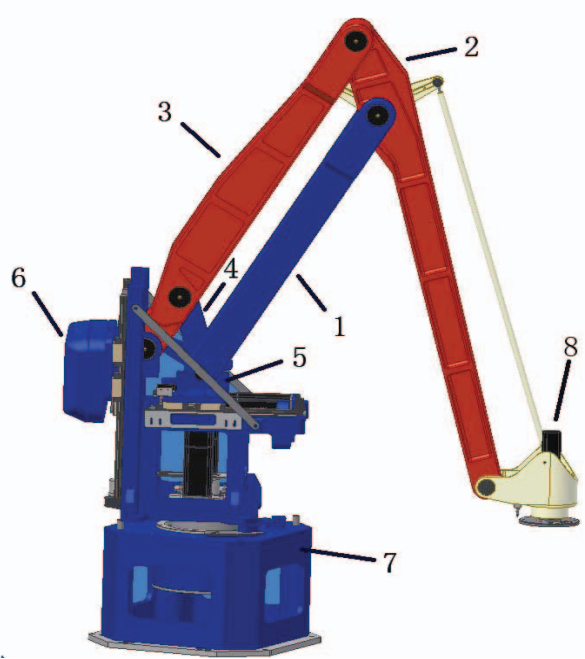
\includegraphics[width=0.4\columnwidth]{alt_robot_arch.png}}
%\hfill
%\subfloat[haptic device with a parallelogram architecture \cite{phantom}.\label{fig:hap_device}]{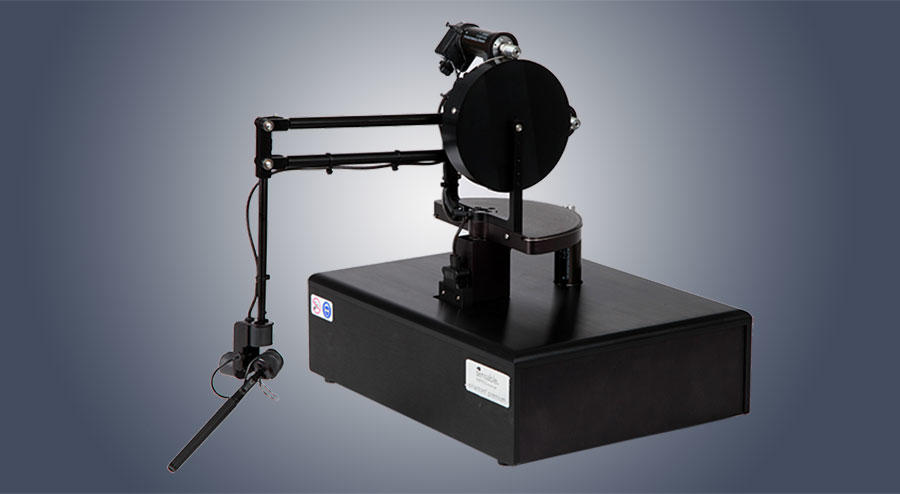
\includegraphics[width=0.5\columnwidth]{phantom.jpg}}

%\subfloat[backdrivable pHRI parallel robot \cite{wen2019kinematically}\cite{9306904}.
%\label{fig:phri_robot}]{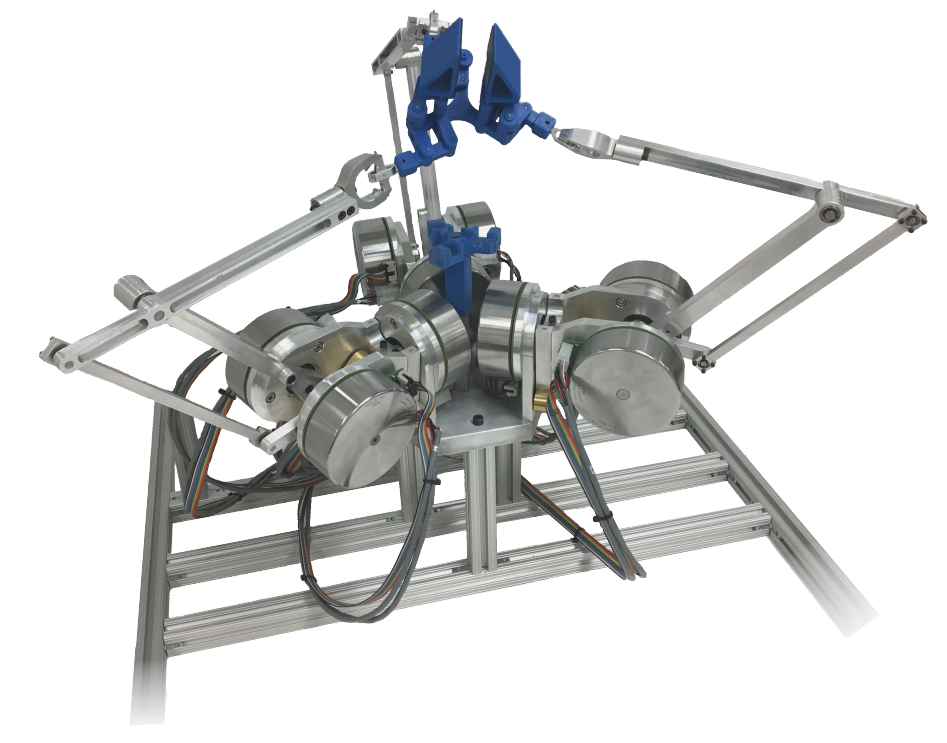
\includegraphics[width=\columnwidth]{proto_keifei.png}}
%\caption{Palletizing robot, haptic device and backdrivable pHRI robot using alternative parallelogram like architectures.}
%\label{fig:alt_arch}
%\end{figure} 
LRT are already used in haptic devices for telesurgery \cite{gosselin2011specification}\cite{perret2014advantages}\cite{baumann1998haptic}\cite{carignan2000closed}. Yet, not all LRT are mechanically backdrivable. For example, a worm gear cannot be driven by its output (through the worm).Table \ref{tab:LRT} shows a list of backdrivable LRT and indicates their advantages and disadvantages for pHRI.
\begin{table}[]
\caption{Comparison of different backdrivable LRT.}
\label{tab:LRT}
\begin{tabularx}{0.5\textwidth}{@{}XXX@{}}
\toprule
LRT type    & Advantages     & Disadvantages                                                                                       \\ \midrule
Spur and helical gears &
  \begin{tabular}[c]{@{}X@{}}High stiffness\\ High torque capability\end{tabular} &
  \begin{tabular}[c]{@{}X@{}}Clearance between\\ teeth\\ (backlash)\end{tabular} \\
\hline
Belt drive &
  \begin{tabular}[c]{@{}X@{}}Transmission over a larger distance\\ No backlash\end{tabular} &
  \begin{tabular}[c]{@{}X@{}}Lower stiffness\\ Slip error\end{tabular} \\
\hline
Chain Drive & High stiffness & \begin{tabular}[c]{@{}X@{}}Clearance between inner links\\ Higher transmission inertia\end{tabular} \\
\hline
Cable (capstan drive) &
  \begin{tabular}[c]{@{}X@{}}Higher stiffness than belt drive\\ No backlash\end{tabular} &
  \begin{tabular}[c]{@{}X@{}}Lower stiffness than chain and gears\\ Slip error\end{tabular} \\ \bottomrule
\end{tabularx}
\end{table}
\par Table \ref{tab:LRT} shows that a capstan drive is a good choice of backdrivable LRT because it has higher stiffness than a belt drive and it has a low backlash like gears or chain drives. This is why it is used in haptic devices \cite{perret2014advantages}\cite{baser2013kinematic}, highly backdrivable collaborative robots \cite{townsend1988effect}\cite{rooks2006harmonious}\cite{phan2014guided} and high precision targeting systems \cite{lu2015development}\cite{lu2012non}\cite{lu2013transmission}\cite{xie2019analytical}. Having low backlash is very important for  robotics applications which require the robot's motors to work in both directions at a high frequency \cite{brooks1990telerobotic}\cite{gealy2019quasi}. However, Table \ref{tab:LRT} also shows that capstan drives have lower stiffness than other LRT such as gears and can be subject to slip error \cite{lu2013transmission}\cite{baser2010theoretical}.\par
In order to alleviate these drawbacks, this article presents a novel capstan architecture that increases the stiffness of the transmission by using grooves on the transmission's pulleys. The grooves increase the friction coefficient between the cable and the pulleys, which makes the transmission stiffer. This concept has already been used in cable transmissions for elevators as described in \cite{gibsonfred} and \cite{hymans2013neuzeitliche} Moreover, the novel capstan drive allows multiple cable arrangements, which further increases the stiffness of the transmission.\par This paper is structured as follows. In Section II and III, the general modelling of a capstan drive and its torsional stiffness are recalled. The theoretical model used here is based on the work of Werkmeister et al.\cite{werkmeister2007theoretical}. Part of this model is also used in \cite{baser2010theoretical}. Section IV explains how grooves etched along the surface of a capstan drive's pulleys can theoretically increase the friction coefficient between the drive's cable and its pulleys thus increasing the overall stiffness of the capstan drive. The use of grooves in capstan drives has already been presented in \cite{lu2012non}. However, this paper presents a novel design for the output pulley of a capstan drive which uses grooves arranged as a multiple helix. This novel design enables different multi-cable arrangements of the capstan drive that can theoretically further increase its torsional stiffness. The novel capstan drive architecture as well as different possible cable arrangements are presented in Section V. The advantages and disadvantages  of each of the proposed arrangements are discussed. Section VI then proposes a method to properly arrange the capstan drive's pulleys during the drive's assembly so that the cables can follow a smooth and continuous path while passing from one pulley to the other. Finally, concluding remarks are made in Section VIII.
\section{Modelling of a capstan drive}
Figure \ref{fig:model_capstan} presents the different elements of the capstan drive model.
\begin{figure}
    \centering
    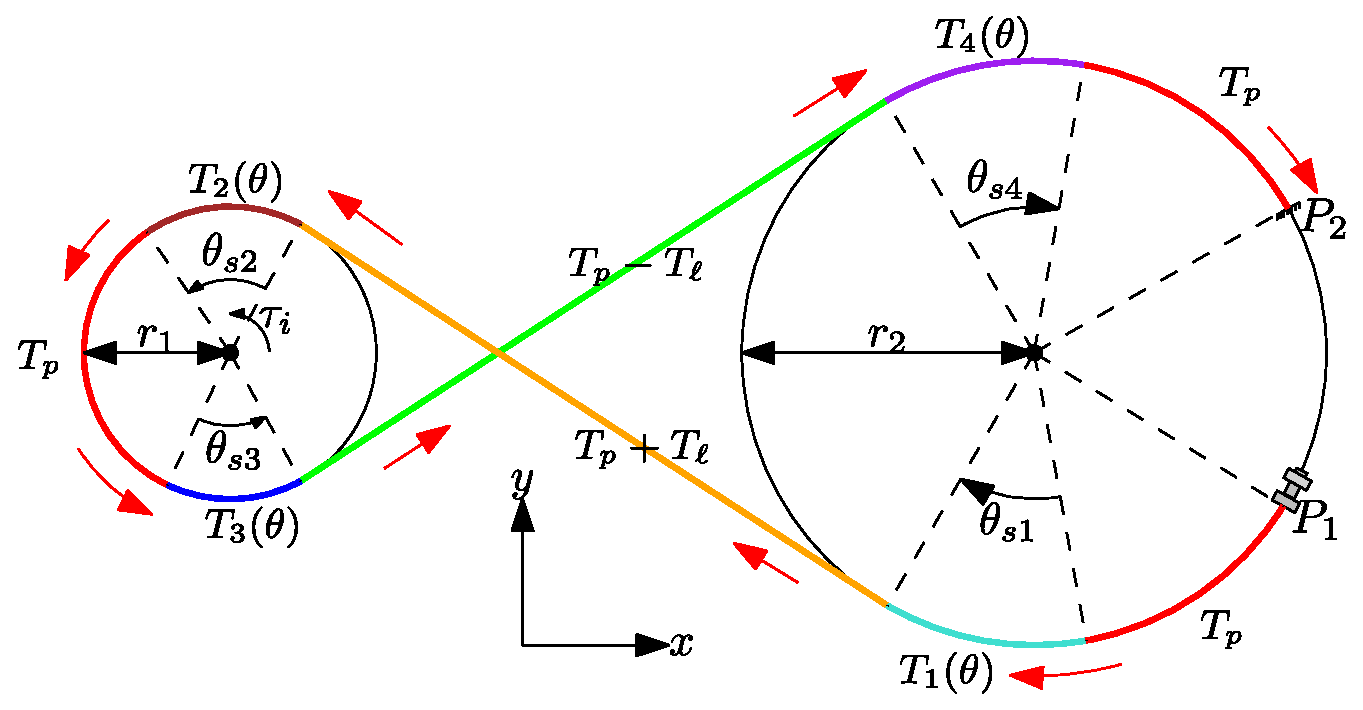
\includegraphics[width=0.46\textwidth]{modelling_of_capstan_drive.eps}
    \caption{Modelling of a capstan drive.}
    \label{fig:model_capstan}
\end{figure}
In figure \ref{fig:model_capstan}, $r_1$ is the radius of the small input pulley while $r_2$ is the radius of the large output pulley. The transmission ratio is given by $R = \frac{r_2}{r_1}$. The cable passes from the large pulley to the small pulley and back to the large pulley in a lemniscate shaped pattern indicated by the red arrows in figure \ref{fig:model_capstan}. A preload tension $T_p$ is applied on the cable by pulling on the cable with a mechanism alike a turnbuckle (at point $P_1$) and by fixing the other end of the cable to the pulley(at point $P_2$).\par
When a torque $\tau_i$ is applied on the input pulley, one side of the cable extends while the other part of the cable shortens. The extension is caused by an increase in the tension in the cable by an amount $T_\ell$ while the contraction of the other part of the cable is caused by a reduction of the tension by an equal amount $T_\ell$. The tension on the taught side becomes $T_p+T_\ell$ while the tension on the loose side becomes $T_p-T_\ell$. The torque balance equation about the axis of rotation of the input pulley can be written as
\begin{align}
    \tau_i - (T_p+T_\ell)r_1 + (T_p-T_\ell)r_1 = 0, \label{eq:first_equation_p0}
\end{align}
which yields
\begin{align}
T_\ell = \frac{\tau_i}{2r_1}.
\label{eq:first_equation}
\end{align}
\par
The tension variations in the cable occur in contact regions between the cable and the pulleys called the slip regions. These regions are represented in figure \ref{fig:model_capstan} with the angles $\theta_{s1}$ to $\theta_{s4}$. Along these slip regions, the cable elongates or shortens due to the applied torque. This local variation in length causes friction between the pulleys and the cable. Figure \ref{fig:friction_fig} illustrates this principle. 
\begin{figure}
    \centering
    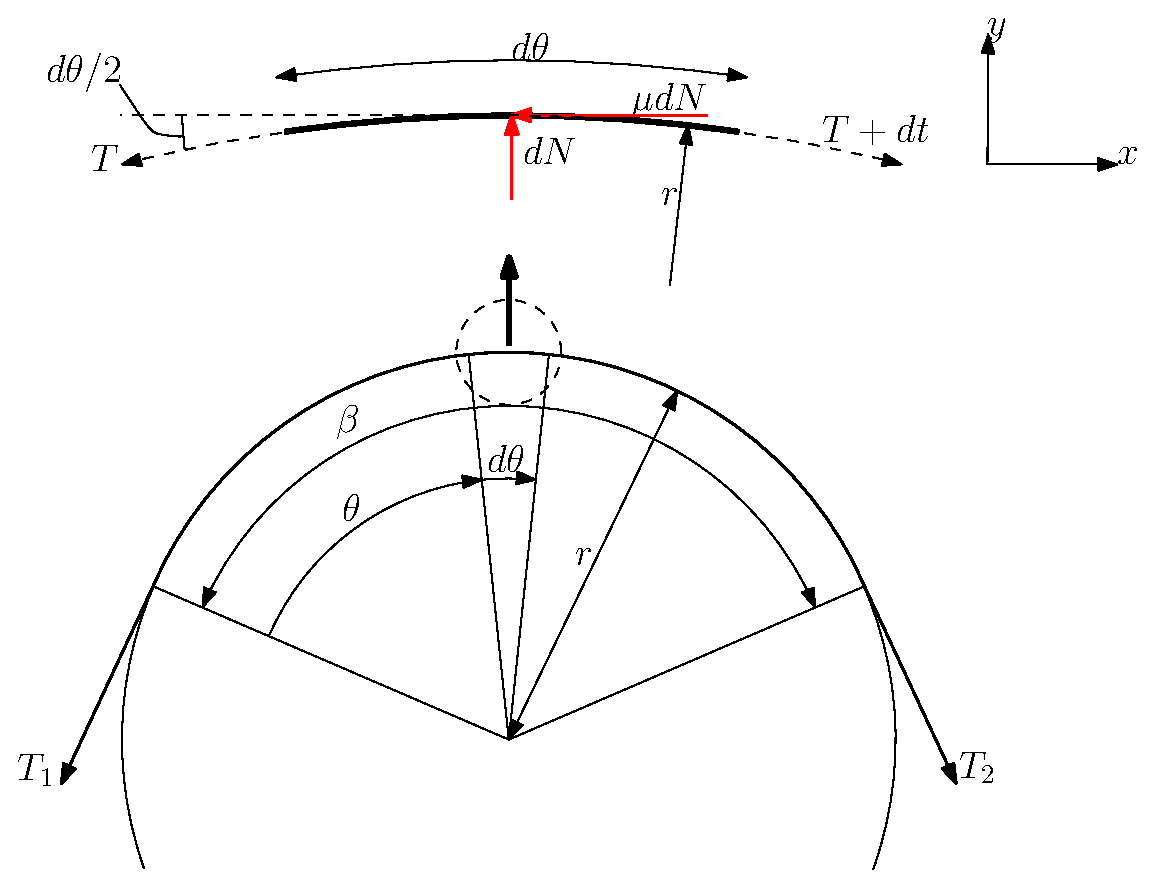
\includegraphics[width = 0.43\textwidth]{capstan_equation.eps}
    \caption{Small segment of the cable pulley interaction.}
    \label{fig:friction_fig}
\end{figure}
\par
Figure \ref{fig:friction_fig} shows a small  segment of a cable lying on the surface of a pulley of radius $r$. The small cable segment is lying on a small angle segment of the pulley $d\theta$. The static friction coefficient between the pulley and the cable is $\mu$. The tension on one end of the small cable segment is $T$ while it is $T+dT$ at the other end. The small tension variation is created by an applied torque on the pulley. The normal force between the small cable segment and the pulley  is $dN$. When torque is applied to the pulley, the pulley surface creates a friction force on the cable segment of $\mu dN$ in the tangential direction of the torque. Calculating the force balance on the cable segment gives 
\begin{align}
    \sum F_x = T\cos\left(\frac{d\theta}{2}\right) - (T+dT)\cos\left(\frac{d\theta}{2}\right) + \mu dN =0,\label{eq:sum_f_x}\\
    \sum F_y = -T\sin\left(\frac{d\theta}{2}\right)-(T+dT)\sin\left(\frac{d\theta}{2}\right)+dN = 0.\label{eq:sum_f_y}
\end{align}
Since $d\theta$ is a small angle and $dT$ is a small tension variation, the following approximations can be made
\begin{align}
    \sin\left(\frac{d\theta}{2}\right)\approx \frac{d\theta}{2},\hquad \cos\left(\frac{d\theta}{2}\right)\approx 1,\hquad dTd\theta \approx 0. 
\end{align}
Applying these approximations to\eqref{eq:sum_f_x} and \eqref{eq:sum_f_y} gives
\begin{align}
    \frac{dT}{T} = \mu d\theta. \label{eq:diff}
\end{align}
In figure \ref{fig:friction_fig}, when the tension varies from $T_1$ to $T_2$ where $T_2>T_1$, the integration over the angle $\beta$ of \eqref{eq:diff} gives
\begin{align} 
\beta = \frac{1}{\mu}\ln\left(\frac{T_2}{T_1}\right).
\label{eq:int_beta}
\end{align}
Angle $\beta$ is referred to as the slip angle of the slip region. Integrating from $T_1$ to a function $T(\theta)$ over the slip region then gives \begin{align}
T(\theta) = T_1e^{\mu\theta},\hquad 0<\theta<\beta.\label{eq:tens_increase}
\end{align}
The same can be said by integrating from the max tension $T_2$ to a smaller tension $T(\theta)$ over the slip region $\beta$, which gives
\begin{align}
T(\theta) = T_2e^{-\mu\theta},\hquad 0<\theta<\beta.\label{eq:tens_decrease}
\end{align}
Applying \eqref{eq:int_beta}, \eqref{eq:tens_increase} and \eqref{eq:tens_decrease} to the slip regions in figure \ref{fig:model_capstan}, one finds
\begin{align}
    T_1(\theta) = T_pe^{\mu\theta},\hquad 0<\theta<\theta_{s1},\hquad \theta_{s1} = \frac{1}{\mu}\ln\left(\frac{T_p+T_\ell}{T_p}\right),\label{eq:Tens1}\\
    T_2(\theta) = (T_p+T_\ell)e^{-\mu\theta},\hquad 0<\theta<\theta_{s2},\hquad \theta_{s2}=\theta_{s1},\label{eq:Tens2}\\
    T_3(\theta) = T_pe^{-\mu\theta},\hquad 0<\theta<\theta_{s3},\hquad \theta_{s3} = \frac{1}{\mu}\ln\left(\frac{T_p}{T_p-T_\ell}\right),\label{eq:Tens3}\\
    T_4(\theta) = (T_p-T_\ell)e^{\mu\theta},\hquad 0<\theta<\theta_{s4},\hquad \theta_{s4} = \theta_{s3}.\label{eq:Tens4}
\end{align}
Equations \eqref{eq:Tens1} to \eqref{eq:Tens4} describe the variation of the tension along the cable. These equations are used in the following section to model the stiffness of a capstan drive.
%%%%%%%%%%%%%%%%%%%%%%%%%%%%%%%%%%%%%%%%%%%%%%%%%%%%%%%%%%%%%%%%%%%%%%
\section{Stiffness model of a capstan drive}
Hooke's law gives the relationship between the tensile force in an elastic object and its strain. The strain of an elastic object is also defined as its variation in length over its original length. Expressing this definition of strain in an infinitesimal form and equating it to Hooke's law, one can then write
\begin{align}
\epsilon \equiv \frac{d\delta}{dL} = \frac{F}{AE}, \Rightarrow d\delta = \frac{FdL}{AE}
\label{eq:complete_short}
\end{align}
where $\epsilon$ is the strain, $d\delta$ is a very small length variation, $dL$ is a very small cable length, $F$ is the tensile force applied on the elastic object, $A$ is the object's  cross section area and $E$ is its Young modulus. Equation \eqref{eq:complete_short} can be integrated to determine the cable deformation.
\par
The  cable deformation $\delta_i$ along the slip region $\theta_{si}$ is equal to the total deformation along the slip region minus the initial deformation caused by the preload.  Using \eqref{eq:complete_short} and using the fact that $dL=rd\theta$, the deformations $\delta_i$ are obtained as 
\begin{align}
    \delta_i = \frac{r}{AE}\left(\int_0^{\theta_{si}}T_i(\theta)d\theta-T_p\int_0^{\theta_{si}}d\theta\right),\hquad i=1,\ldots ,4 \label{eq:int_deform_i_theta}
\end{align}
where $r = r_2$ for $\theta_{s1}$ and $\theta_{s4}$ and $r = r_1$ for $\theta_{s2}$ and $\theta_{s3}$.
Applying \eqref{eq:int_deform_i_theta} to the slip angle $\theta_{s1}$ gives
\begin{align}
    \delta_1 = \frac{T_pr_2}{AE}\left(\int_0^{\theta_{s1}}e^{\mu\theta} d\theta-\int_0^{\theta_{s1}}d\theta\right), \\
    = \frac{T_pr_2}{AE}\left(\frac{1}{\mu}\left(e^{\mu\theta{s1}} -1\right)-\theta_{s1}\right),\\
    =\frac{r_2}{\mu AE}\left(T_\ell-T_p\ln\left(\frac{T_p+T_\ell}{T_p}\right)\right)\label{eq:defo1}.
\end{align}
Similarly for $\delta_2$ to $\delta_4$, one obtains 
\begin{align}
    \delta_2=\frac{r_1}{\mu AE}\left(T_\ell-T_p\ln\left(\frac{T_p+T_\ell}{T_p}\right)\right),\label{eq:defo2}\\
    \delta_3= \frac{r_1}{\mu AE}\left(T_\ell-T_p\ln\left(\frac{T_p}{T_p-T_\ell}\right)\right),\label{eq:defo3}\\
    \delta_4 =\frac{r_2}{\mu AE}\left(T_\ell-T_p\ln\left(\frac{T_p}{T_p-T_\ell}\right)\right).\label{eq:defo4}
\end{align}
Some cable deformation also occurs in the cable sections which are not in contact with the pulleys. These cable sections are here called the free sections and the deformation along these sections is obtained by integrating \eqref{eq:complete_short} which gives
\begin{align}
\delta_{f1} = \frac{T_p+T_\ell}{AE}\int_0^{L_f}dL=\frac{T_p+T_\ell}{AE}L_f,\label{eq:defof1}\\
\delta_{f2}=\frac{T_p-T_\ell}{AE}\int_0^{L_f}dL=\frac{T_p-T_\ell}{AE}L_f,\label{eq:defof2}
\end{align}
where $\delta_{f1}$ and $\delta_{f2}$ are the deformations on the tight and slack side respectively and $L_f$ is the length of the free parts of the cable which are not in contact with the pulleys.
\par
 The compliance of the different cable sections can be defined as the absolute value of the variation in deformation of the cable as a function of the applied load. Mathematically, this means that the compliance of the different cable sections can be obtained by differentiating the deformation expressions in \eqref{eq:defo1} to \eqref{eq:defof2} with respect to $T_\ell$. Furthermore, since compliance is the inverse of stiffness, one can easily obtain the stiffness of the different cable sections. For the slip regions, this gives
 \begin{align}
     C_{si}=\left|\frac{d\delta_{si}}{dT_\ell}\right|,\hquad i = 1,\ldots ,4,\label{eq:simple_stiff_1}\\
     \Rightarrow C_{s1} = \frac{r_2}{AE\mu}\left(\frac{T_\ell}{T_p+T_\ell}\right) = \frac{1}{K_{s1}}\\
     \Rightarrow C_{s2} = \frac{r_1}{AE\mu}\left(\frac{T_\ell}{T_p+T_\ell}\right)= \frac{1}{K_{s2}}\\
     \Rightarrow C_{s3} =
     \frac{r_1}{AE\mu}\left(\frac{T_\ell}{T_p-T_\ell}\right)= \frac{1}{K_{s3}}\\
     \Rightarrow C_{s4} =
     \frac{r_2}{AE\mu}\left(\frac{T_\ell}{T_p-T_\ell}\right)= \frac{1}{K_{s1}}\label{eq:simple_stiff_4}
 \end{align}
 For the stiffnesses of the free sections of the cable, one obtains
 \begin{align}
     K_{f1}=K_{f2}=\frac{AE}{L_f}
 \end{align}
 The total stiffness of the capstan transmission is obtained by combining the individual stiffnesses of the cable segments along the transmission. The stiffness elements $K_{s1},K_{f_1}$ and $K_{s2}$ form a serial combination of springs. The same can be said for $K_{s3},K_{f_2}$ and $K_{s4}$. The two serial springs groups are in parallel to one another meaning that the total stiffness of the transmission can be written as 
 \begin{align}
     K = K_1 + K_2,
 \end{align}
 where
 \begin{align}
     K_1 = \frac{1}{\frac{1}{K_{s1}}+\frac{1}{K_{f1}}+\frac{1}{K_{s2}}},\\
     K_2 = \frac{1}{\frac{1}{K_{s3}}+\frac{1}{K_{f2}}+\frac{1}{K_{s4}}}.
 \end{align}
 The total stiffness $K$ represents the linear stiffness of the transmission. Since a capstan drive is a torsional element, a better indicator of its stiffness is the drive's torsional stiffness when one of its pulleys is held rigidly. The torsional stiffness $K_t$ of the capstan drive when the small pulley is held rigidly and  a torque $\tau$ is applied on the large pulley, causing an angular displacement $\alpha$, is then given by
 \begin{align}
     \tau = K_t\alpha. \label{eq:rot_stiff}
 \end{align}
 The relationship between $K_t$ and $K$ is obtained by writing
 \begin{align}
    \frac{\tau_D}{r_2} = K\delta \label{eq:lin_stiff}\\
     \alpha = \frac{\delta}{r_2} \label{eq:rot_disp}.
 \end{align}
 Equation \eqref{eq:lin_stiff} gives the relationship between a torque $\tau$ applied on the large pulley  of radius $r_2$ and the total linear displacement $\delta$ when the small pulley is held tightly. Equation \eqref{eq:rot_disp} gives the relationship between the total linear displacement of the cable and the angular displacement $\alpha$ of the large pulley of radius $r_2$. Using these two equations with \eqref{eq:rot_stiff} yields
 \begin{align}
     K_t = Kr_2^2. 
 \end{align}
The following section shows how placing the capstan transmission's cable into grooves helps to increase the coefficient of friction between the cable and the pulleys and therefore the transmission's stiffness.

\section{Influence of grooves on the capstan drive stiffness}
 Analyzing the equations for the stiffness of the different cable sections of a capstan drive ((32) to (35)), one can clearly see that all the stiffness terms are proportional to the coefficient of friction. Therefore, Increasing the coefficient of friction between the cable and the pulleys is an effective way to increase the overall stiffness of the transmission. Typically, the coefficient of friction is a property that is only dependant on the nature of the materials at the friction interface. However, like for a v-belt drive, by changing the geometry of the interface between two surfaces, it is possible to change the apparent coefficient of friction. Figure \ref{fig:distib_force} illustrates how circular grooves help to increase the coefficient of friction between the cable and the capstan drive pulleys.\\
 \begin{figure}
    \centering
    %\subfloat[Uniform distribution.\label{fig:uniform_force}]{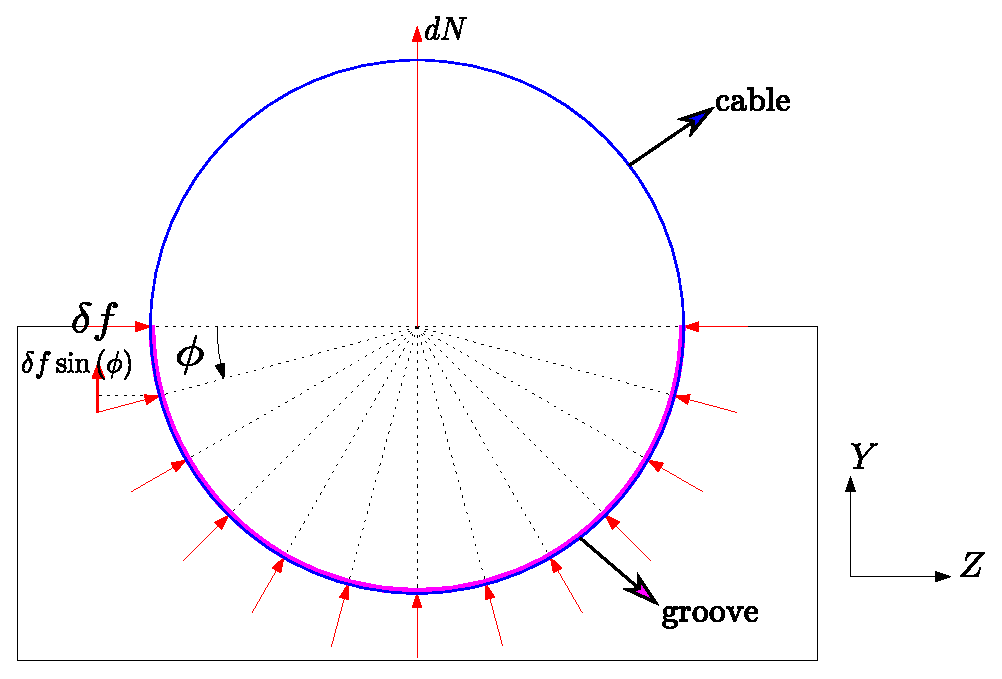
\includegraphics[width =0.8\columnwidth]{distribution_de_force_cable.eps}}\\    
    %\subfloat[General distribution.\label{fig:general_force}]
    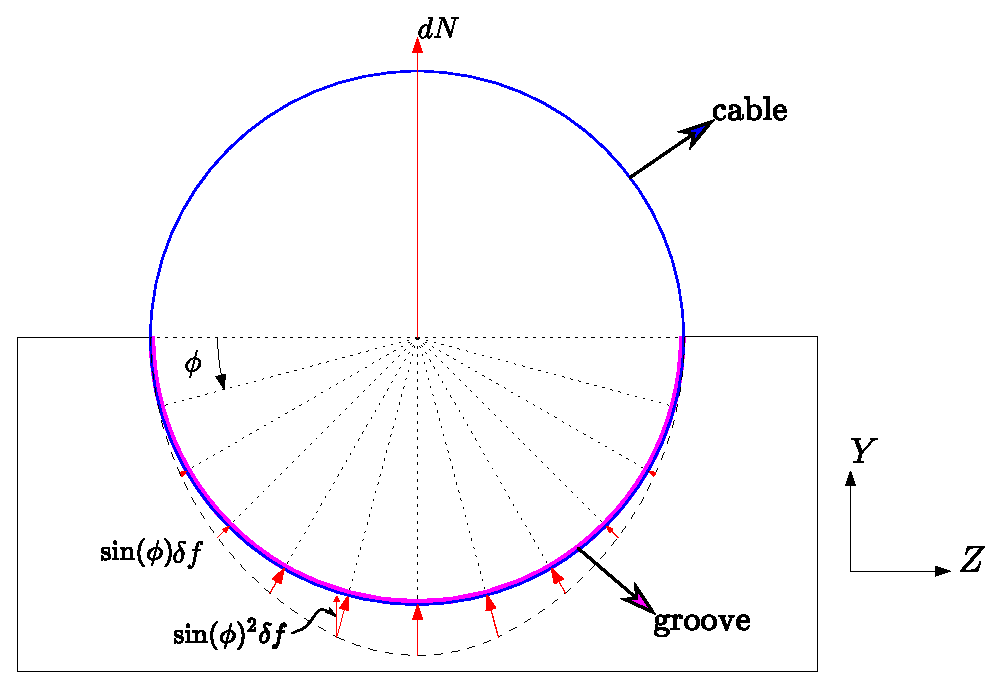
\includegraphics[width =0.8\columnwidth]{distribution_tension_gen.eps}
    \caption{Distribution of the normal force along the cross-section interface between the cable and the pulleys.}
    \label{fig:distib_force}
\end{figure}
 The illustrations in figure \ref{fig:distib_force} show the distribution of the normal force occurring between a small section of the cable and a pulley groove. In figure \ref{fig:distib_force}, the distribution of the normal force is considered to proportional to the sin of the angle $\phi$. This normal force distribution makes it so that the normal force at the bottom of the groove is maximum while the normal force at the sides of the  The figure shows the cross section of the interface which is perpendicular to the plane shown in figure \ref{fig:friction_fig}. The equivalent normal force between the small cable segment and the pulley segment is noted $dN$ and can be mathematically obtained as 
 \begin{align}
     dN = \int_0^\pi \delta f\sin{\phi}d\phi = 2\delta f,
     \label{eq:small_normforce}
 \end{align}
 where $\phi$ is the variable angle along the interface cross section and $\delta f$ is a unit force quantity. Applying Coulomb's law of static friction to the cross-section in figure \ref{fig:uniform_force} gives 
 \begin{align}
     dF_f = \int_0^\pi\mu df d\theta=\pi\mu df, \label{eq:small_friction}
 \end{align}
 where $dF_f$ is the friction force between the cable segment and the cable pulley. Combining  \eqref{eq:small_normforce} and \eqref{eq:small_friction} gives
 \begin{align}
     dF_f=\mu'dN=\frac{\pi\mu}{2}dN,\label{eq:eff_fric}
 \end{align}
 where $\mu'$ is the effective coefficient of friction between the cable and the pulley grooves. Equation \eqref{eq:eff_fric} shows that, when considering a uniform distribution along the cross section of the cable pulley interface, grooves can help to increase the effective friction coefficient by a factor of $\pi/2$. However, this force distribution along the interface arc is very unlikely considering the fact that local normal force around the middle of the cross-section arc is likely larger than the one at each extremity of the cross-section arc. Considering this, figure \ref{fig:general_force} shows how the force could be distributed along the cross-section arc if a general force distribution function $g(\phi)$ is considered. The effective friction coefficient given this consideration is then obtained by
 \begin{align}
     dN = \delta f I_1(\phi) = \delta f\int_0^{\pi}g(\phi)\sin\phi d\phi,\\
     dF_f = \mu\delta f I_2(\phi) = \mu\delta_f\int_0^\pi\mu g(\phi)d\phi.\\
     dF_f =\mu'dN= \frac{\mu I_2(\phi)}{I_1(\phi)}dN.
 \end{align}
 For any type of positive distribution function $g(\phi)$, the ratio of $\frac{I_2(\phi)}{I_1(\phi)}$ will always be greater than 1. This means that a groove can only increase the effective friction coefficient between the cable and the pulleys of a capstan drive and will therefore make it stiffer. 
\\ 
 The following section presents a novel capstan drive architecture that takes advantage of the increased effective friction coefficient of grooved pulleys and uses multiple grooves on its output pulley in order to allow different cable arrangements which further increase the stiffness of the drive.
%%%%%%%%%%%%%%%%%%%%%%%%%%%%%%%%%%%%%%%%%%%%%%%%%%%%%%%%%%%%%%%%%%%%%%
\subsection{Second-Level Heading}

The next level of heading is also boldface with upper and lower case letters. 
The heading is flushed left with the left margin. The spacing to the next heading is two line spaces.

%%%%%%%%%%%%%%%%%%%%%%%%%%%%%%%%%%%%%%%%%%%%%%%%%%%%%%%%%%%%%%%%%%%%%%
\subsubsection{Third-Level Heading.}

The third-level of heading follows the style of the second-level heading.


%%%%%%%%%%%%%%%%%%%%%%%%%%%%%%%%%%%%%%%%%%%%%%%%%%%%%%%%%%%%%%%%%%%%%%
\section{Use of SI Units}

An ASME paper should use SI units.  When preference is given to SI units, the U.S. customary units may be given in parentheses or omitted. When U.S. customary units are given preference, the SI equivalent {\em shall} be provided in parentheses or in a supplementary table. 

%%%%%%%%%%%%%%%%%%%%%%%%%%%%%%%%%%%%%%%%%%%%%%%%%%%%%%%%%%%%%%%%%%%%%%
\section{Footnotes\protect\footnotemark}
\footnotetext{Examine the input file, asme2ej.tex, to see how a footnote is given in a head.}

Footnotes are referenced with superscript numerals and are numbered consecutively from 1 to the end of the paper\footnote{Avoid footnotes if at all possible.}. Footnotes should appear at the bottom of the column in which they are referenced.


%%%%%%%%%%%%%%%%%%%%%%%%%%%%%%%%%%%%%%%%%%%%%%%%%%%%%%%%%%%%%%%%%%%%%%
\section{Mathematics}

Equations should be numbered consecutively beginning with (1) to the end of the paper, including any appendices.  The number should be enclosed in parentheses and set flush right in the column on the same line as the equation.  An extra line of space should be left above and below a displayed equation or formula. \LaTeX\ can automatically keep track of equation numbers in the paper and format almost any equation imaginable. An example is shown in Eqn.~(\ref{eq_ASME}). The number of a referenced equation in the text should be preceded by Eqn.\ unless the reference starts a sentence in which case Eqn.\ should be expanded to Equation.

\begin{equation}
f(t) = \int_{0_+}^t F(t) dt + \frac{d g(t)}{d t}
\label{eq_ASME}
\end{equation}

%%%%%%%%%%%%%%%%%%%%%%%%%%%%%%%%%%%%%%%%%%%%%%%%%%%%%%%%%%%%%%%%%%%%%%
\section{Figures}
\label{sect_figure}

All figures should be positioned at the top of the page where possible.  All figures should be numbered consecutively and centered under the figure as shown in Fig.~\ref{figure_ASME}. All text within the figure should be no smaller than 7~pt. There should be a minimum two line spaces between figures and text. The number of a referenced figure or table in the text should be preceded by Fig.\ or Tab.\ respectively unless the reference starts a sentence in which case Fig.\ or Tab.\ should be expanded to Figure or Table.


%%%%%%%%%%%%%%%%%%%%%%%%%%%%%%%%%%%%%%%%%%%%%%%%%%%%%%%%%%%%%%%%%%%%%%
%%%%%%%%%%%%%%%% begin figure %%%%%%%%%%%%%%%%%%%
\begin{figure}[t]
\begin{center}
\setlength{\unitlength}{0.012500in}%
\begin{picture}(115,35)(255,545)
\thicklines
\put(255,545){\framebox(115,35){}}
\put(275,560){Beautiful Figure}
\end{picture}
\end{center}
\caption{The caption of a single sentence does not have period at the end}
\label{figure_ASME} 
\end{figure}
%%%%%%%%%%%%%%%% end figure %%%%%%%%%%%%%%%%%%% 
%%%%%%%%%%%%%%%%%%%%%%%%%%%%%%%%%%%%%%%%%%%%%%%%%%%%%%%%%%%%%%%%%%%%%%

In the following subsections, I have inserted figures that have been provided by authors in order to demonstrate what to avoid.  In each case the authors provided figures that are 3.25in wide and 600dpi in the .tif graphics format.  The papers containing these figures have been held from production due to their poor quality. 

%%%%%%%%%%%%%%%%%%%%%%%%%%%%%%%%%%%%%%%%%%%%%%%%%%%%%%%%%%%%%%%%%%%%%%
\subsection{The 1st Example of Bad Figure}

%%%%%%%%%%%%%%%% begin figure %%%%%%%%%%%%%%%%%%%
%%% 3.34in is the maximum width you can have for a figure
\begin{figure} 
\centerline{\psfig{figure=figure/FMANU_MD_05_1107_11.ps,width=3.34in}}
\caption{Example taken from a paper that was held from production because the image quality is poor.  ASME sets figures captions in 8pt, Helvetica Bold.}
\label{fig_example1.ps}
\end{figure}
%%%%%%%%%%%%%%%% end figure %%%%%%%%%%%%%%%%%%%

In order to place the figure in this template using MSWord, select Insert Picture from File,and use wrapping that is  top and bottom.  Make sure the figure is 3.25in wide.
 
Figure~`\ref{fig_example1.ps}
was taken from a recent paper that was held from publication, because the text is fuzzy and unreadable.  It was probably obtained by taking a screen shot of the computer output of the authors software.  This means the original figure was 72dpi (dots per inch) on a computer screen.  There is no way to improve the quality such a low resolution figure.
 
In order to understand how poor the quality of this figure is, please zoom in slightly, say to 200\%.  Notice that while the font of the paper is clear at this size, the font in the figures is fuzzy and blurred.  It is impossible to make out the small symbol beside the numbers along the abscissa of the graph.  Now consider the labels Time and Cost.  They are clearly in fonts larger that the text of the article, yet the pixilation or rasterization, associated with low resolution is obvious. This figure must be regenerated at higher resolution to ensure quality presentation.

The poor quality of this figure is immediately obvious on the printed page, and reduces the impact of the research contribution of the paper, and in fact detracts from the perceived quality of the journal itself.



%%%%%%%%%%%%%%%%%%%%%%%%%%%%%%%%%%%%%%%%%%%%%%%%%%%%%%%%%%%%%%%%%%%%%%
\subsection{The 2nd Example of Bad Figure}

%%%%%%%%%%%%%%%% begin figure %%%%%%%%%%%%%%%%%%%
\begin{figure} 
\centerline{\psfig{figure=figure/FMANU_MD_05_1272_5.ps,width=3.34in}}
\caption{While this figures is easily readable at a double column width of 6.5in, when it is shrunk to 3.25in column width the text is unreadable.   This paper was held from production.}
\label{fig_example2.ps}
\end{figure}
%%%%%%%%%%%%%%%% end figure %%%%%%%%%%%%%%%%%%%

Figure~\ref{fig_example2.ps}
demonstrates a common problem that arises when a figure is scaled down fit a single column width of 3.25in.  The original figure had labels that were readable at full size, but become unreadable when scaled to half size.  This figure also suffers from poor resolution as is seen in the jagged lines the ovals that form the chain.

This problem can be addressed by increasing the size of the figure to a double column width of 6.5in, so the text is readable.  But this will not improve the line pixilation, and a large low resolution figure is less desirable than a small one.  This also significantly expands the length of the paper, and may cause it to exceed the JMD nine page limit.  Additional pages require page charges of \$200 per page.  It is best to regenerate the figure at the resolution that ensures a quality presentation.


%%%%%%%%%%%%%%%%%%%%%%%%%%%%%%%%%%%%%%%%%%%%%%%%%%%%%%%%%%%%%%%%%%%%%%
\subsection{The 3rd Example of Bad Figure}
%%%%%%%%%%%%%%%% begin figure %%%%%%%%%%%%%%%%%%%
\begin{figure} 
%\centerline{\psfig{figure=figure/FMANU_MD_04_1274_13.ps,width=3.34in}}
\centerline{\psfig{figure=figure/FMANU_MD_04_1274_13.ps,width=3.25in}}
\caption{Another example of a figure with unreadable text.  Even when the paper was expanded to double column width the text as shown in Fig.~\ref{fig_example4.ps} was of such low quality that the paper was held from production.}
\label{fig_example3.ps}
\end{figure}
%%%%%%%%%%%%%%%% end figure %%%%%%%%%%%%%%%%%%%

%%%%%%%%%%%%%%%% begin figure %%%%%%%%%%%%%%%%%%%
%%% the maximum width in double column is 6.85in
\begin{figure*} 
\centerline{\psfig{figure=figure/FMANU_MD_04_1274_13.ps,width=6.85in}}
\caption{A figure expanded to double column width the text from Figure~\ref{fig_example3.ps}}
\label{fig_example4.ps}
\end{figure*}
%%%%%%%%%%%%%%%% end figure %%%%%%%%%%%%%%%%%%%
An author provided the high resolution image 
in Fig.~\ref{fig_example3.ps}
that was sized to a single column width of 3.25in.  Upon seeing the poor quality of the text, the publisher scaled the image to double column width as shown in Fig.~\ref{fig_example4.ps} 
at which point it took half of a page.  The publisher went on to do this for all eight figures generating four pages of figures that the author did not expect. ASME stopped production of the paper even with the larger figures due to the pixilation of the font.

Clearly the text in this figure is unreadable, and it is doubtful that the author can print the output in a way that it is readable.  This is a problem that the author must solve, not the publisher. 

As you might expect, I have many more examples, but in the end the author is the best judge of what is needed in each figure.  ASME simply requires that the image meet a minimum standard for font and line quality, specifically the font should be the appropriate size and not be blurred or pixilated, and that lines should be the appropriate weight and have minimal, preferably no, pixilation or rasterization.


%%%%%%%%%%%%%%%%%%%%%%%%%%%%%%%%%%%%%%%%%%%%%%%%%%%%%%%%%%%%%%%%%%%%%%
\section{Tables}

%%%%%%%%%%%%%%%%%%%%%%%%%%%%%%%%%%%%%%%%%%%%%%%%%%%%%%%%%%%%%%%%%%%%%%
%%%%%%%%%%%%%%% begin table   %%%%%%%%%%%%%%%%%%%%%%%%%%
\begin{table}[t]
\caption{Figure and table captions do not end with a period}
\begin{center}
\label{table_ASME}
\begin{tabular}{c l l}
& & \\ % put some space after the caption
\hline
Example & Time & Cost \\
\hline
1 & 12.5 & \$1,000 \\
2 & 24 & \$2,000 \\
\hline
\end{tabular}
\end{center}
\end{table}
%%%%%%%%%%%%%%%% end table %%%%%%%%%%%%%%%%%%% 
%%%%%%%%%%%%%%%%%%%%%%%%%%%%%%%%%%%%%%%%%%%%%%%%%%%%%%%%%%%%%%%%%%%%%%

All tables should be numbered consecutively  and centered above the table as shown in Table~\ref{table_ASME}. The body of the table should be no smaller than 7 pt.  There should be a minimum two line spaces between tables and text.


%%%%%%%%%%%%%%%%%%%%%%%%%%%%%%%%%%%%%%%%%%%%%%%%%%%%%%%%%%%%%%%%%%%%%%
\section{Citing References}

%%%%%%%%%%%%%%%%%%%%%%%%%%%%%%%%%%%%%%%%%%%%%%%%%%%%%%%%%%%%%%%%%%%%%%
The ASME reference format is defined in the authors kit provided by the ASME.  The format is:

\begin{quotation}
{\em Text Citation}. Within the text, references should be cited in  numerical order according to their order of appearance.  The numbered reference citation should be enclosed in brackets.
\end{quotation}

The references must appear in the paper in the order that they were cited.  In addition, multiple citations (3 or more in the same brackets) must appear as a `` [1-3]''.  A complete definition of the ASME reference format can be found in the  ASME manual \cite{asmemanual}.

The bibliography style required by the ASME is unsorted with entries appearing in the order in which the citations appear. If that were the only specification, the standard {\sc Bib}\TeX\ unsrt bibliography style could be used. Unfortunately, the bibliography style required by the ASME has additional requirements (last name followed by first name, periodical volume in boldface, periodical number inside parentheses, etc.) that are not part of the unsrt style. Therefore, to get ASME bibliography formatting, you must use the \verb+asmems4.bst+ bibliography style file with {\sc Bib}\TeX. This file is not part of the standard BibTeX distribution so you'll need to place the file someplace where LaTeX can find it (one possibility is in the same location as the file being typeset).

With \LaTeX/{\sc Bib}\TeX, \LaTeX\ uses the citation format set by the class file and writes the citation information into the .aux file associated with the \LaTeX\ source. {\sc Bib}\TeX\ reads the .aux file and matches the citations to the entries in the bibliographic data base file specified in the \LaTeX\ source file by the \verb+\bibliography+ command. {\sc Bib}\TeX\ then writes the bibliography in accordance with the rules in the bibliography .bst style file to a .bbl file which \LaTeX\ merges with the source text.  A good description of the use of {\sc Bib}\TeX\ can be found in \cite{latex, goosens} (see how two references are handled?).  The following is an example of how three or more references \cite{latex, asmemanual,  goosens} show up using the \verb+asmems4.bst+ bibliography style file in conjunction with the \verb+asme2ej.cls+ class file. Here are some more \cite{art, blt, ibk, icn, ips, mts, mis, pro, pts, trt, upd} which can be used to describe almost any sort of reference.

%%%%%%%%%%%%%%%%%%%%%%%%%%%%%%%%%%%%%%%%%%%%%%%%%%%%%%%%%%%%%%%%%%%%%%
\section{Conclusions}
The only way to ensure that your figures are presented in the ASME Journal of Mechanical Design in the way you feel is appropriate and meets the requirement for quality presentation is for you to prepare a double column version of the paper in a form similar to that used by the Journal.

This gives you the opportunity to ensure that the figures are sized appropriately, in particular that the labels are readable and match the size of the text in the journal, and that the line weights and resolutions have no pixilation or rasterization.  Poor quality figures are immediately obvious on the printed page, and this detracts from the perceived quality of the journal.

I am pleased to provide advice on how to improve any figure, but this effort must start with a two-column version of the manuscript. Thank you in advance for your patience with this effort, it will ensure quality presentation of your research contributions.



%%%%%%%%%%%%%%%%%%%%%%%%%%%%%%%%%%%%%%%%%%%%%%%%%%%%%%%%%%%%%%%%%%%%%%
\section{Discussions}
This template is not yet ASME journal paper format compliant at this point.
More specifically, the following features are not ASME format compliant.
\begin{enumerate}
\item
The format for the title, author, and abstract in the cover page.
\item
The font for title should be 24 pt Helvetica bold.
\end{enumerate}

\noindent
If you can help to fix these problems, please send us an updated template.
If you know there is any other non-compliant item, please let us know.
We will add it to the above list.
With your help, we shall make this template 
compliant to the ASME journal paper format.


%%%%%%%%%%%%%%%%%%%%%%%%%%%%%%%%%%%%%%%%%%%%%%%%%%%%%%%%%%%%%%%%%%%%%%
\begin{acknowledgment}
This work was supported by the Natural Sciences and Engineering Research Council of Canada (NSERC) and by the
Canada Research Chair Program.
\end{acknowledgment}

%%%%%%%%%%%%%%%%%%%%%%%%%%%%%%%%%%%%%%%%%%%%%%%%%%%%%%%%%%%%%%%%%%%%%%
% The bibliography is stored in an external database file
% in the BibTeX format (file_name.bib).  The bibliography is
% created by the following command and it will appear in this
% position in the document. You may, of course, create your
% own bibliography by using thebibliography environment as in
%
% \begin{thebibliography}{12}
% ...
% \bibitem{itemreference} D. E. Knudsen.
% {\em 1966 World Bnus Almanac.}
% {Permafrost Press, Novosibirsk.}
% ...
% \end{thebibliography}

% Here's where you specify the bibliography style file.
% The full file name for the bibliography style file 
% used for an ASME paper is asmems4.bst.
\bibliographystyle{asmems4}

% Here's where you specify the bibliography database file.
% The full file name of the bibliography database for this
% article is asme2e.bib. The name for your database is up
% to you.
%\bibliography{asme2e}
\bibliography{./bibliography/asme2e}
%%%%%%%%%%%%%%%%%%%%%%%%%%%%%%%%%%%%%%%%%%%%%%%%%%%%%%%%%%%%%%%%%%%%%%
\appendix       %%% starting appendix
\section*{Appendix A: Head of First Appendix}
Avoid Appendices if possible.

%%%%%%%%%%%%%%%%%%%%%%%%%%%%%%%%%%%%%%%%%%%%%%%%%%%%%%%%%%%%%%%%%%%%%%
\section*{Appendix B: Head of Second Appendix}
\subsection*{Subsection head in appendix}
The equation counter is not reset in an appendix and the numbers will
follow one continual sequence from the beginning of the article to the very end as shown in the following example.
\begin{equation}
a = b + c.
\end{equation}

\end{document}
